\documentclass[a4paper,10pt,fleqn]{article}
\ifdefined\print
  \usepackage[print]{sicpsetup}
\else
  \usepackage{sicpsetup}
\fi
\date{\today}

%
\author{Daniel Perez}
\sicptitle{5.3と5.4}
%
\begin{document}
\maketitle
%
\section*{概要}
今回の2章を掛けて, レジスターマシンを用いた評価機の設計と実装に%
ついて説明する.

まず, 5.3では評価機を作る際に必要になるメモリの管理について説明する.
メモリをどう表現するのかと, ガーベージコレクションの役割りと1つの%
実装について説明する.

メモリを使える状況にしたあとに, 実際の評価機の実装に入る. そこで, 4章で%
作った評価機を変えて, Schemeで評価する仕様から, レジスターマシンを使って%
評価する仕様に変える.
%
\setcounter{section}{5}
%
\setcounter{subsection}{2}
\subsection{記憶域の割当とガベージコレクション}
5.4では, レジスターマシンを使ってSchemeの評価機を%
作成する. そのために, メモリーを抽象化した方が良いので,
リスト構造として表現したメモリーとそのメモリを操作するための%
抽象化を作る.

リストで表現したメモリを作るために, 主に2つの問題点がある.
\begin{enumerate}
\item コンピュータのメモリで表現できるものだけでどのように%
  リスト構造を表現することができるか.
\item メモリがなるべくいっぱいにならなようにどうすれば良いのか.
\end{enumerate}
%
まず1について説明し, そのあとガーベージコレクションの説明で%
2について説明する.
%
\subsubsection{ベクタとしてのメモリ}
コンピュータのメモリはユーニックなアドレスを持つブロックで分かれている.
基本的にブロックに値を入れるための操作とブロックからその値を取り出す%
ための操作が準備されていることが多い. また, メモリのアドレスも
データとして扱われていて, そのアドレスで演算などを行うことができる.

メモリを表現するために, ベクターというデータ構造を用いる.
ベクターはコンパウンドデータで, 添字を用いて定数時間で要素を%
取り出せるようになっている. メモリの操作を表すために,
次の2つのプロシジャを用いる.

\begin{lstlisting}[basicstyle=\footnotesize]
(vector-ref <vector> <n>)
(vector-set! <vector> <n> <value)
\end{lstlisting}
\paragraph{Lispのデータ構造の表現}
ベクターを用いてリスト構造に使うペアを表すことができる.
メモリが\lstinline{the-cars}と\lstinline{the-cdrs}という2つの%
ベクターで分かれているとする. ペアはその2つのベクターの添字として%
表すことができる. また, 数字や記号を表す方法も必要となる. そのために,
型のついたポインターを用いることができる. 例えば, \lstinline{n4}は
4という整数を表し, \lstinline{p5}はインデックス5のペアを表す. また,
\lstinline{e0}は空のリストを表す.
%
\begin{figure}[h]
  \centering
  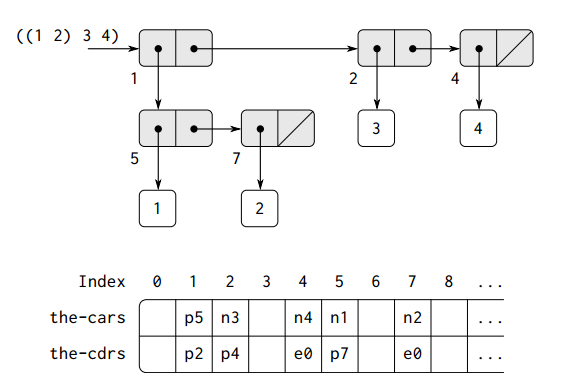
\includegraphics[height=6cm,width=12cm]{imgs/box-and-pointer.png}
\end{figure}
%
\paragraph{リストの基本操作}
操作を実装するために, \lstinline{the-cars}と\lstinline{the-cdrs}レジスターを用いる.
また, \lstinline{vector-ref}と\lstinline{vector-set!}という操作が使えることを%
前提とする. それを用いて,
%
\begin{lstlisting}[basicstyle=\footnotesize]
(assign <reg 1 > (op car) (reg <reg 2 >))
(assign <reg 1 > (op cdr) (reg <reg 2 >))
\end{lstlisting}
%
を次のように実装できる.
%
\begin{lstlisting}[basicstyle=\footnotesize]
(assign <reg 1 > (op vector-ref) (reg the-cars) (reg <reg 2 >))
(assign <reg 1 > (op vector-ref) (reg the-cdrs) (reg <reg 2 >))
\end{lstlisting}

\lstinline{set-car!}と\lstinline{set-cdr!}についても同じく実装できる.

また, 次に使える添字を常に指している\lstinline{free}というレジスターが%
存在するとする. それらを用いて,

\begin{lstlisting}[basicstyle=\footnotesize]
(assign <reg 1 > (op cons) (reg <reg 2 >) (reg <reg 3 >))
\end{lstlisting}
を次のように実装できる.
\begin{lstlisting}[basicstyle=\footnotesize]
(perform
  (op vector-set!) (reg the-cars) (reg free) (reg <reg 2 >))
(perform
  (op vector-set!) (reg the-cdrs) (reg free) (reg <reg 3 >))
(assign <reg 1 > (reg free))
(assign free (op +) (reg free) (const 1))
\end{lstlisting}

また, \lstinline{eq?}を次のように

\begin{lstlisting}[basicstyle=\footnotesize]
(op eq?) (reg <reg 1 >) (reg <reg 2 >)
\end{lstlisting}

で実装できる.
%
\subsubsection{無限のメモリの幻想を維持する}
以上紹介した構造では, リスト構造を表現することができるが,
メモリーが無限にあるという前提になってしまう. 実際の%
コンピュータでは, メモリが有限なので, メモリを使い切らない方法%
を考える必要がある. そのために, 使わなくなった結果などを消して%
そのメモリの部分を再利用できるようにする. その方法は
ガーベージコレクションという.

\paragraph{stop-and-copyガーベージコレクター}
ここで, \lstinline{root}というレジスターが%
現在アクセスできるすべてのデータの情報を持つ%
データ構造を指しているとする.

メモリで2つで分ける. 現在使っているデータは%
\lstinline{the-cars}と\lstinline{the-cdrs}とし,
使われていないメモリは\lstinline{new-cars}と\lstinline{new-cdrs}とする.

現在使っているメモリがいっぱいになると, 使っているデータのみ
使われていないメモリにコピーし, 現在のメモリをすべて空にする.

\begin{figure}[h]
  \centering
  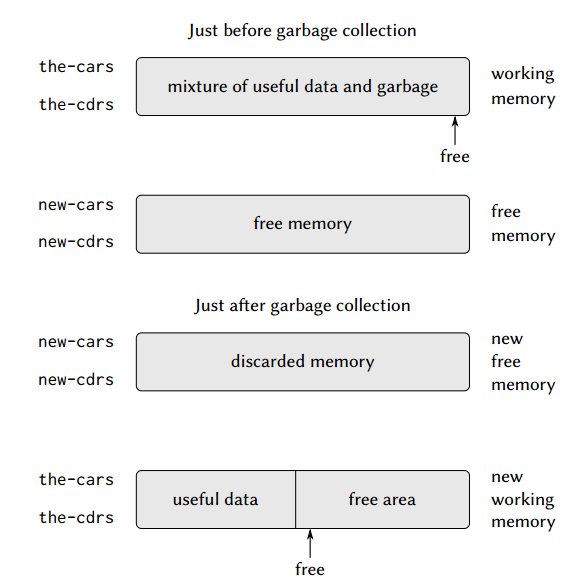
\includegraphics[height=6cm,width=8cm]{imgs/stop-and-copy.png}
\end{figure}


%
\subsection{明示的制御評価機}
4.1章では, Schemeのインタープリタをどうすれば\lstinline{eval}と%
\lstinline{apply}で表すのかについて説明した. ここで実装する%
明示的制御評価機で, 評価における引数の管理などをどのようにレジスタ%
とスタックで表現できるかについて説明する.

今回実装する評価機は, スタックと7つのレジスタを持つ. レジスタは
\lstinline{exp} (評価される式), \lstinline{env} (評価の環境),
\lstinline{val} (評価の結果), \lstinline{continue} (再帰のため),
\lstinline{proc}, \lstinline{arg1}, \lstinline{unev} (コンビネーションの評価).
%
\subsubsection{明示制御評価機のコア}
評価機の中心は\lstinline{eval-dispatch}で始まる%
命令のシーケンスである. 4.1の\lstinline{eval}プロシジャー%
に相当する部分になっている. そこで, \lstinline{exp}に入っている%
式を\lstinline{env}の環境で実行し, 結果を\lstinline{val}に%
保存する. 実装は次のようにできる.

\begin{lstlisting}[basicstyle=\footnotesize,caption=]
eval-dispatch
  (test (op self-evaluating?) (reg exp))
  (branch (label ev-self-eval))
  (test (op variable?) (reg exp))
  (branch (label ev-variable))
  (test (op quoted?) (reg exp))
  (branch (label ev-quoted))
  (test (op assignment?) (reg exp))
  (branch (label ev-assignment))
  (test (op definition?) (reg exp))
  (branch (label ev-definition))
  (test (op if?) (reg exp))
  (branch (label ev-if))
  (test (op lambda?) (reg exp))
  (branch (label ev-lambda))
  (test (op begin?) (reg exp))
  (branch (label ev-begin))
  (test (op application?) (reg exp))
  (branch (label ev-application))
  (goto (label unknown-expression-type))
\end{lstlisting}

\paragraph{単純式の評価}
サブ式のない式の場合, 結果を\lstinline{val}に入れて, あとは%
\lstinline{continue}に入っているエントリーポイントで%
実行を続ける. 例えば, \lstinline{variable}の場合は次のように%
実装できる.

\begin{lstlisting}[basicstyle=\footnotesize]
ev-variable
  (assign val (op lookup-variable-value) (reg exp) (reg env))
  (goto (reg continue))
\end{lstlisting}
%
\paragraph{プロシジャー適用の評価}
\lstinline{eval}プロシジャーでは, オペレータを評価し,
再帰的にオペランドを評価していき,
結果を\lstinline{apply}に渡すことによって評価していた.
今回も同じアプローチを使い, 再帰は\lstinline{goto}命令で
表現し, 値が必要なレジスタの値を一時的に保存するには, スタックを用いる.
オペレータはの評価は次のように実装できる.

\begin{lstlisting}[basicstyle=\footnotesize]
ev-application
  (save continue)
  (save env)
  (assign unev (op operands) (reg exp))
  (save unev)
  (assign exp (op operator) (reg exp))
  (assign continue (label ev-appl-did-operator))
  (goto (label eval-dispatch))
ev-appl-did-operator
  (restore unev) ; the operands
  (restore env)
  (assign argl (op empty-arglist))
  (assign proc (reg val)) ; the operator
  (test (op no-operands?) (reg unev))
  (branch (label apply-dispatch))
  (save proc)
\end{lstlisting}

%
\subsubsection{シーケンスの評価と末尾再帰}
今回の評価機の\lstinline{ev-sequence}は4.1の評価機%
の\lstinline{eval-sequence}に相当するもので,
プロシジャーのボディと\lstinline{begin}で定義されたような%
シーケンスを評価する. 実装は次のようにできる.

\begin{lstlisting}[basicstyle=\footnotesize,caption=]
ev-sequence
  (assign exp (op first-exp) (reg unev))
  (test (op last-exp?) (reg unev))
  (branch (label ev-sequence-last-exp))
  (save unev)
  (save env)
  (assign continue (label ev-sequence-continue))
  (goto (label eval-dispatch))
ev-sequence-continue
  (restore env)
  (restore unev)
  (assign unev (op rest-exps) (reg unev))
  (goto (label ev-sequence))
ev-sequence-last-exp
  (restore continue)
  (goto (label eval-dispatch))
\end{lstlisting}

このシーケンスにこれ以上式が残っていない時は, \lstinline{continue}を%
スタックから戻し, \lstinline{eval-dispatch}に飛ぶ.



%
\end{document}
